% the hard case: prior exactly half a turn away (theta = 180 degrees), h0 = 0, h3 = beta
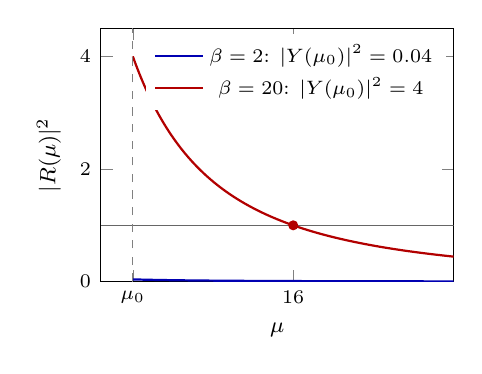
\begin{tikzpicture}
  \begin{axis}[width=0.5\textwidth, height=4.8cm, xmin=4, xmax=26, ymin=0, ymax=4.5,
      xlabel={$\mu$}, ylabel={$|R(\mu)|^2$}, xtick={6,16}, xticklabels={$\mu_0$,$16$},
      legend style={at={(0.98,0.98)}, anchor=north east, font=\scriptsize, draw=none},
      tick label style={font=\scriptsize}, label style={font=\footnotesize}, samples=200, domain=6:26]
    \addplot[thick, blue!70!black] {4/(x+4)^2};
    \addplot[thick, red!70!black] {400/(x+4)^2};
    \draw[black!60] (axis cs:4,1) -- (axis cs:26,1);
    \draw[gray, dashed] (axis cs:6,0) -- (axis cs:6,4.5);
    \addplot[only marks, mark=*, mark size=1.6pt, red!70!black] coordinates {(16,1)};
    \legend{{$\beta = 2$: $|Y(\mu_0)|^2 = 0.04$}, {$\beta = 20$: $|Y(\mu_0)|^2 = 4$}}
  \end{axis}
\end{tikzpicture}\hspace{1em}
\begin{tikzpicture}[scale=1.5]
  \draw[thick] (0,0) circle (1);
  \fill[blue!70!black] (0:1) circle (1.4pt) node[below right] {$R_0$};
  \fill[blue!40] (180:1) circle (1.4pt) node[below left] {$-R_0$};
  \fill[orange!80!black] (90:1) circle (1.4pt) node[above] {$\bar R = E_3$};
  \fill[red!70!black] (11.54:1) circle (1.5pt) node[above right, font=\scriptsize] {$Y + \tau R_0$};
  \fill[red!70!black] (168.46:1) circle (1.5pt) node[above left, font=\scriptsize] {$Y - \tau R_0$};
  \draw[-{Stealth[length=2mm]}, orange!80!black] (0,0) -- (0,0.2) node[right, font=\scriptsize] {$Y$};
  \node[font=\scriptsize, align=center] at (0,-1.35) {$\beta = 2$: two maximizers,\\ rotations by $\pm 23.1^\circ$};
\end{tikzpicture}
